\section{Ejemplo de seccion}

Esto son ejemplos de como poner negritas y esas cosas:

Some of the \textbf{greatest}
discoveries in \underline{science} 
were made by \textbf{\textit{accident}}.

Esto otro una foto:

{\centering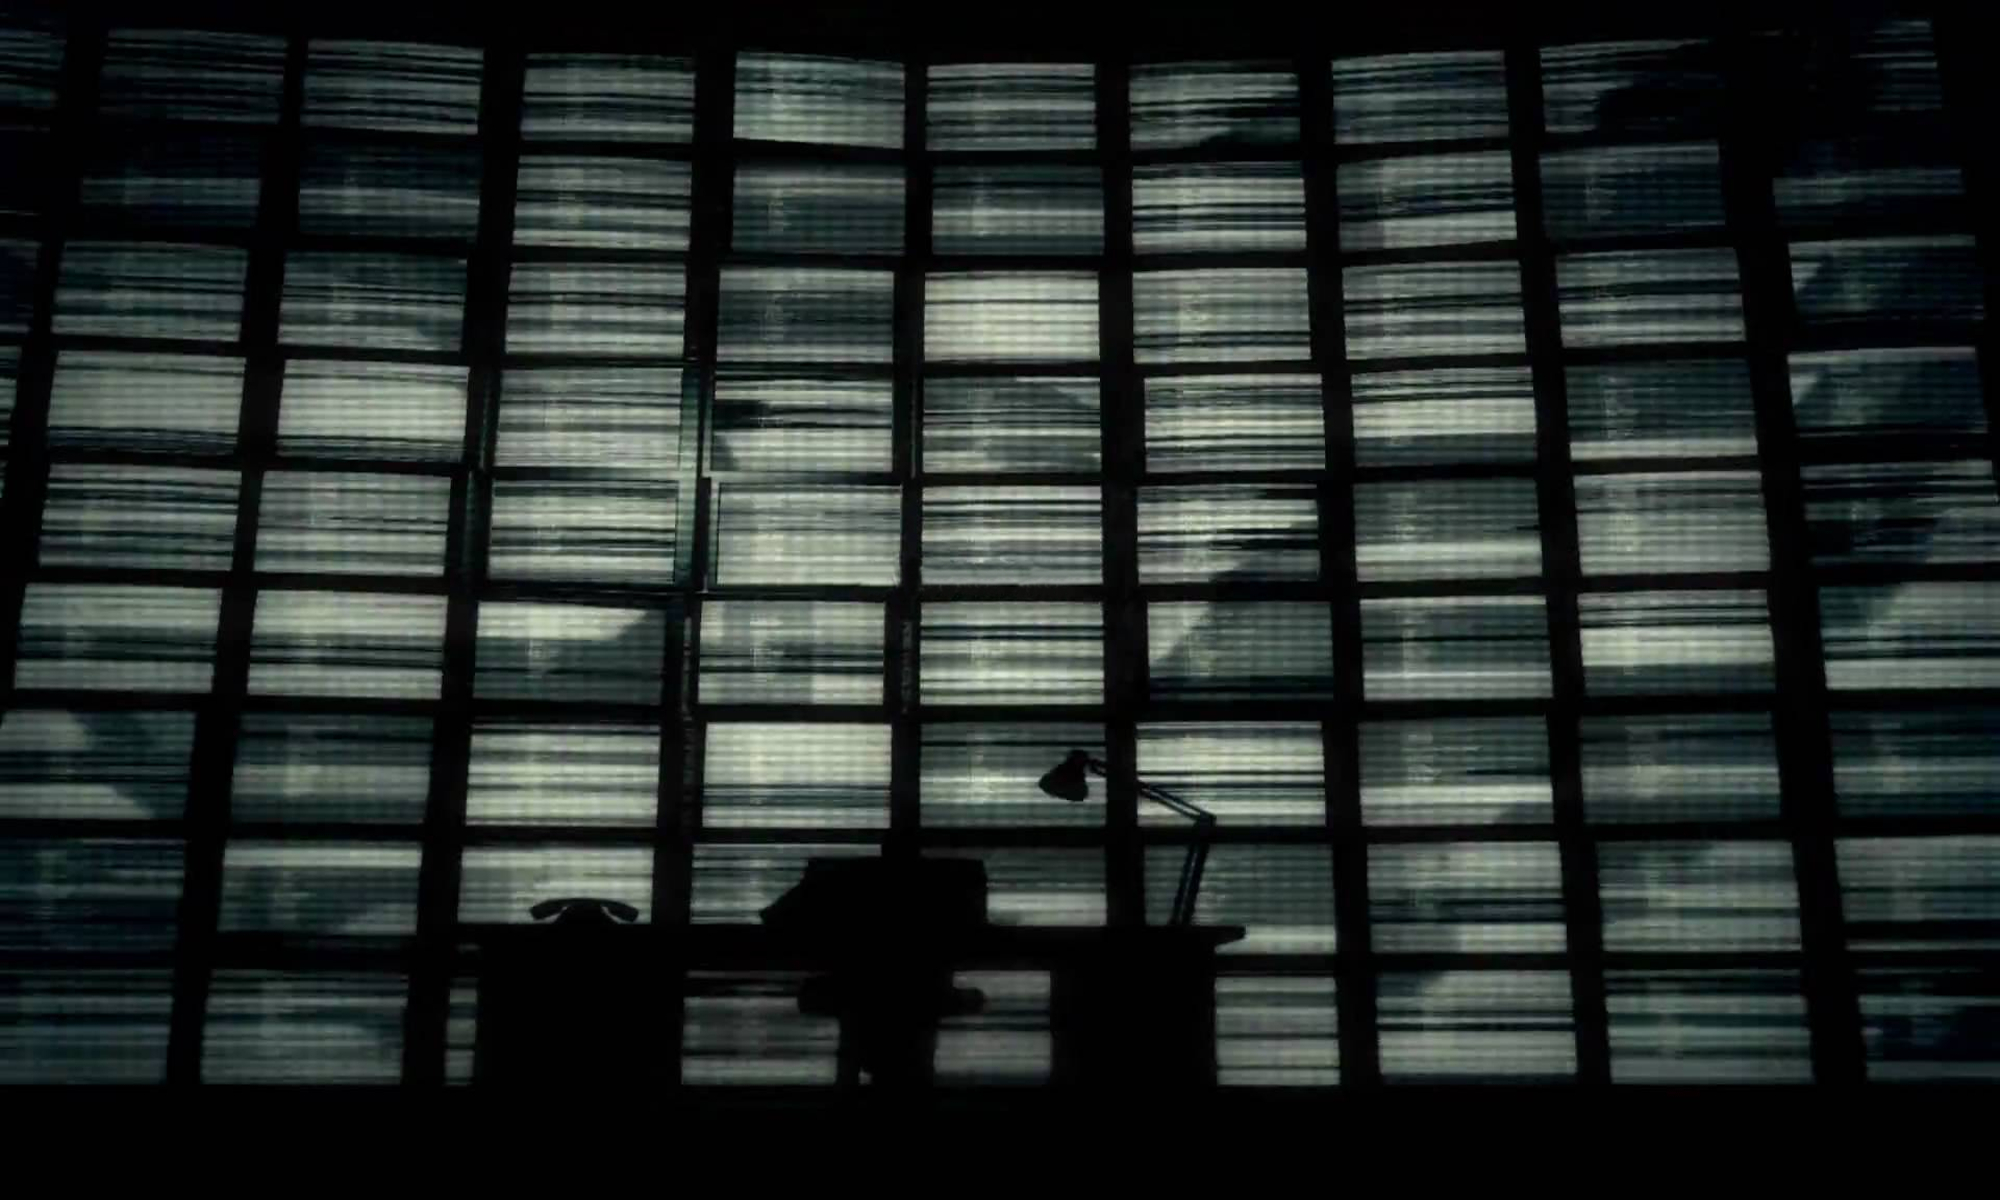
\includegraphics[width=\textwidth]{prueba}}


Centrada y tal.

Esto otro son listas numeradas y no numeradas:

\begin{itemize}
  \item The individual entries are indicated with a black dot, a so-called bullet.
  \item The text in the entries may be of any length.
\end{itemize}

\begin{enumerate}
  \item This is the first entry in our list
  \item The list numbers increase with each entry we add
\end{enumerate}
\pagebreak
